\section{Primitive Operations}
    Here we reorganize algorithms in \cite{repsum} into a user-friendly set of
    primitive operations on an indexed type. Two simple original algorithms
    relating to the index of an indexed type are given in Section
    \ref{sec:primitiveops_index}. Theoretical summaries of algorithms (with
    some improvements) from \cite{repsum} are provided in Sections
    \ref{sec:primitiveops_update}, \ref{sec:primitiveops_deposit},
    \ref{sec:primitiveops_renormalize}, \ref{sec:primitiveops_reduce}. Section
    \ref{sec:primitiveops_convert} provides an original algorithm (with an
    improved error bound) to obtain the value represented by an indexed type.
    Sections \ref{sec:primitiveops_error} and \ref{sec:primitiveops_limits}
    extend analysis in \cite{repsum} to the new algorithms.
  \subsection{Index}
    \label{sec:primitiveops_index}
    When operating on indexed types it is sometimes necessary to compute their
    index. Algorithm \ref{alg:iindex} yields the index of an indexed type in
    constant time.

    \begin{samepage}
    \begin{alg}
      Given an indexed type $Y$, calculate its index $I$
      \begin{algorithmic}[1]
        \Require
          \Statex ${Y_0}_P \in (\epsilon^{-1}  2^{a_{I}}, 2  \epsilon^{-1}  2^{a_I})$
          where $a_I$ is defined in \eqref{eq:a}
        \Function{IIndex}{Y}
          \State \Return $\lfloor(e_{\max} + p - \exp({Y_0}_P) - W + 1)/W\rfloor$
          \Comment{Index $I$ of $Y$}
        \EndFunction
        \Ensure
          \Statex Returned result $I$ is the index of $Y$.
      \end{algorithmic}
      \label{alg:iindex}
    \end{alg}
    \end{samepage}

    Note that the floor function is necessary in Algorithm \ref{alg:iindex} to
    account for the case of $Y$ with index $0$, which has $\exp({Y_0}_P) =
    2^{e_{\max}}$ as discussed in Section \ref{sec:indexed_overflow}.  This
    uses the assumption that $\frac{p+1}{2} < W < p-2$, so $3 < p - W + 1 < W.$

    Another useful operation is, given some $x \in \F$, to find the unique bin
    $(a_J, b_J]$ such that $2^{b_J} > |x| \geq 2^{a_J}$. Algorithm
    \ref{alg:index} yields such a $J$ in constant time.
    Note that, for $x=0$ or very small values $x < 2^{a_{i_{max}}}$,
    we simply return the least bin
    since values smaller than the least bin will not be accumulated.

    \begin{samepage}
    \begin{alg}
      Given $x \in \F$, calculate $J$ such that $2^{b_J} > |x| \geq 2^{a_J}$.
      \begin{algorithmic}[1]
        \Require $i_{max}$ is defined in \eqref{eq:imax},
          $a_J$ is defined in \eqref{eq:a}.
        \Function{Index}{x}
          \If {$x = 0$} \State \Return $i_{max}$ \EndIf
          \State \Return $\min(i_{max}, \lfloor(e_{\max} - \exp(x))/W\rfloor)$
          \Comment{Index $J$ of $x$}
        \EndFunction
        \Ensure
          \Statex The bin $(a_{J}, b_{J}]$ satisfies $2^{b_{J}} > |x| \geq 2^{a_{J}}$ when
          $|x| \geq 2^{a_{i_{max}}}$, and $J=i_{max}$ otherwise.
      \end{algorithmic}
      \label{alg:index}
    \end{alg}
     \end{samepage}

  \subsection{Deposit}
    \label{sec:primitiveops_deposit}
    The deposit operation (here referred to as Algorithm \ref{alg:deposit},
    which deals with overflow, unlike a simpler version described in the
    ``Extract $K$ first bins'' Section (lines 18-20) of Algorithm $6$ in
    \cite{repsum}) is used to extract the slices of a floating point number and
    add them to the appropriate accumulators of an indexed type.

    Algorithm \ref{alg:depositrestricted} deposits floating point numbers in
    the case that there is no overflow (the indexed type has an index greater
    than 0).

      \begin{samepage}
      \begin{alg}
        Extract slices of $x \in \F$, where $|x| < 2^{b_I}$, in bins $(a_I,
        b_I], ..., (a_{I + K - 1}, b_{I + K - 1}]$ and add to indexed type $Y$.
        Here, $(r | 1)$ represents the result of setting the last bit of the
        significand ($m_{p - 1}$) of floating point number $r$ to 1. This is a
        restatement of lines 18-20 of Algorithm $6$ in \cite{repsum}.
        \begin{algorithmic}[1]
          \Require
          \Statex No overflow occurs.
          \Statex Operations are performed in some ``to nearest'' rounding mode
          (no specific tie breaking behavior is required).
          \Statex $|x| < 2^{b_I}$.
          \Statex ${Y_k}_P \in (\epsilon^{-1}  2^{a_{I + k}}, 2  \epsilon^{-1}  2^{a_{I + k}})$ at all times. (The carry fields ${Y_k}_C$ will be used to ensure this in Algorithm \ref{alg:renorm})
          \Function{DepositRestricted}{K, x, Y}
            \State $r = x$ \label{alg:depositrestricted:rgetsx}
            \For{$k = 0 \To (K - 2)$} \label{alg:depositrestricted:loop}
              \State $S = {Y_k}_P + (r | 1)$ \label{alg:depositrestricted:split}
              \State $q = S - {Y_k}_P$
              \State ${Y_k}_P = S$
              \State $r = r - q$\label{alg:depositrestricted:endsplit}
            \EndFor
            \State ${Y_{K - 1}}_P = {Y_{K - 1}}_P + (r | 1)$
          \EndFunction
          \Ensure
          \Statex The amount added to ${Y_k}_P$ by this algorithm is exactly $d(x, I + k)$.
        \end{algorithmic}
        \label{alg:depositrestricted}
      \end{alg}
      \end{samepage}

      The last bit of $r$ is set to break ties when rounding ``to nearest'' so
      that the amount added to ${Y_k}_P$ does not depend on the size of
      ${Y_k}_P$ so far. The following theorem proves the ``Ensure'' claim at
      the end of Algorithm \ref{alg:depositrestricted}.

    \begin{samepage}
      \begin{thm}
        Let $Y$ be an $K$-fold indexed type of index $I$. Assume that we run
        Algorithm \ref{alg:depositrestricted} on $Y$ and some $x \in \F$, $|x|
        < 2^{b_I}$. If all requirements of the algorithm are satisfied, then
        the amount added to ${Y_k}_P$ is exactly $d(x, I + k)$.
        \label{thm:ddepositrestricted}
      \end{thm}
    \end{samepage}

      \begin{proof}
        Throughout the proof, assume that the phrase ``for all $k$'' means
        ``for all $k \in \{0, ..., K - 1\}$.'' Assume also that $r_k$ and $S_k$
        refer to the value of $r$ and $S$ after executing line
        \ref{alg:depositrestricted:split} in the $k^{th}$ iteration of the
        loop. Finally, assume ${Y_k}_P$ refers to the initial value of
        ${Y_k}_P$ and $S_k$ refers to the final value of ${Y_k}_P$. Therefore,
        $S_k - {Y_k}_P$ is the amount added to ${Y_k}_P$.

        Note that lines
        \ref{alg:depositrestricted:split}-\ref{alg:depositrestricted:endsplit}
        correspond to Algorithm 4 of \cite{repsum}.  Therefore, if
        $\ulp({Y_k}_P) = \ulp(S_k)$ and $\ulp(r_k) < 0.5\ulp({Y_k}_P)$,
        Corollary 3 of \cite{repsum} applies and we have that
        $S_k - {Y_k}_P \in \ulp({Y_k}_P)\Z \in 2^{a_{I + k} + 1}\Z$
        and that $|r_{k + 1}| \leq 0.5\ulp({Y_k}_P) = 2^{a_{I + k}}$.

        As it is assumed
        ${Y_k}_P, S_k \in (\epsilon^{-1}  2^{a_{I + k}}, 2  \epsilon^{-1}  2^{a_{I + k}})$,
        we have $\ulp(S_k) = \ulp({Y_k}_P)$ for all $k$.

        We show $|r_k| \leq 2^{b_{I + k}} = 2^{a_{I + k - 1}}$ for all $k$ inductively.
        As a base case, $r_0 = x$ (from line \ref{alg:depositrestricted:rgetsx}) so $|r_0| = |x| < 2^{b_{I}}$.
        As an inductive step, assume $|r_k| \leq 2^{b_{I + k}}$. We must show $\ulp(r_k) < 0.5\ulp({Y_k}_P)$.

        By Theorem \ref{thm:underflowufp} we have that ${Y_k}_P$ is normalized
        and therefore $\ulp({Y_k}_P) = 2^{a_{I + k} + 1}$.
        If $r_k$ is normalized, then because 
        \(
            \ulp(r_k) \leq 2^{1 - p}|r_k| \leq 2^{b_{I + k} - (p - 1)} = 2^{a_{I + k} + W - (p - 1)},
        \)
        and $W < p - 2$, we have $\ulp(r_k) \leq 2^{a_{I + k} - 1} < 0.5\ulp({Y_k}_P)$.
        (This case is considered in \cite{repsum}).
        If $r_k$ is denormalized, $\ulp(r_k) = 2^{e_{\min} - p + 1}$
        since the unit in the last place of a denormalized number is always equal to $2^{e_{\min} - p + 1}$.
        Using \eqref{eq:binmin},
        \(
            \ulp(r_k)
                = 2^{e_{\min} - p + 1} \leq 2^{e_{\min} - p + 1 + ((e_{\max} - e_{\min} + p - 1) \mod W)}
                = 2^{a_{i_{\max}} - 1} \leq 2^{a_{I + k} - 1} < 0.5\ulp({Y_k}_P).
        \)

        Therefore we have $\ulp(r_k) < 0.5\ulp({Y_k}_P)$. Thus, Corollary 3 of
        \cite{repsum} applies and we have that $|r_{k + 1}| \leq
        0.5\ulp({Y_k}_P) = 2^{a_{I + k}}$. This completes the induction.

        Next, we show $S_k - {Y_k}_P = \roundtonearestinfty(r_k, a_{I + k} + 1)$. As Corollary 3 of \cite{repsum} applies for all $k$, then $S_k - {Y_k}_P \in 2^{a_{I + k} + 1}\Z$. By Theorem 3 of \cite{repsum}, $r_{k + 1} = r_k - (S_k - {Y_k}_P)$. Since $|r_{k + 1}| \leq 2^{a_{I + k}}$, we consider two cases.

        If $|r_k - (S_k - {Y_k}_P)| < 2^{a_{I + k}}$, then $S_k - {Y_k}_P = \roundtonearestinfty(r_k, a_{I + k} + 1)$.

        If $|r_k - (S_k - {Y_k}_P)| = 2^{a_{I + k}}$, then $S_k - {Y_k}_P \in \{r_k + 2^{a_{I + k}},  r_k - 2^{a_{I + k}}\}$.
        As $S_k = \fl({Y_k}_P + (r_k|1))$, we have $|S_k - {Y_k}_P - (r_k|1)| \leq 0.5\ulp(S_k) = 2^{a_{I + k}}$.  As $\ulp(S_k) = \ulp({Y_k}_P) = 2^{a_{I + k} + 1}$, we also have that $r_k \in 2^{a_{I + k}}\Z$  and because $\ulp(r_k) < 2^{a_{I + k}}$, $|(r_k|1) - r_k| > 0$ (with $(r_k|1) - r_k$ taking the same sign as $r_k$).
        If $r_k > 0$, then $(S_k - {Y_k}_P) = r_k + 2^{a_{I + k}}$ (otherwise we will have $|S_k - {Y_k}_P - (r_k|1)| = |r_k - 2^{a_{I + k}} - (r_k|1)| > 2^{a_{I + k}}$).
        If $r_k < 0$, then $(S_k - {Y_k}_P) = r_k - 2^{a_{I + k}}$ (otherwise we will have $|S_k - {Y_k}_P - (r_k|1)| = |r_k + 2^{a_{I + k}} - (r_k|1)| > 2^{a_{I + k}}$). Therefore, $S_k - {Y_k}_P = \roundtonearestinfty(r_k, a_{I + k} + 1)$.

        We can now show $r_{k + 1} = x - \sum\limits_{i = 0}^{I + k}d(x, i)$ and $S_k - {Y_k}_P = d(x, I + k)$ for all $k$ by induction on $k$.

        In the base case, $S_0 - {Y_0}_P = \roundtonearestinfty(r_0, a_I + 1) = \roundtonearestinfty(x, a_I + 1)$. As $|x| < 2^{b_I}$, Lemma \ref{lem:dmiddle} implies $S_0 - {Y_0}_P = d(x, I)$. By Theorem 3 of \cite{repsum}, $r_1 = r_0 - (S_0 - {Y_0}_P) = x - d(x,I)$. By assumption and  \eqref{eq:a} and \eqref{eq:b}, $|x| < 2^{b_I} \leq 2^{a_{i}}$ for all $i \in \{0, ..., I - 1\}$, and therefore by Lemma \ref{lem:dzero}, $r_1 = x - \sum\limits_{i = 0}^Id(x, i)$.

        In the inductive step, assume $r_{k + 1} = x - \sum\limits_{i = 0}^{I + k}d(x, i)$. Then by definition,

        \begin{equation*}
          S_{k + 1} - {Y_{k + 1}}_P = \roundtonearestinfty(r_{k + 1}, a_{I + k + 1} + 1) = \roundtonearestinfty\bigl(x - \sum\limits_{i = 0}^{I + k}d(x, i), a_{I + k + 1} + 1\bigr) = d(x, I + k + 1)
        \end{equation*}

        And by Theorem 3 of \cite{repsum},
        \begin{equation*}
          r_{k + 2} = r_{k + 1} - (S_{k + 1} - {Y_{k + 1}}_P) = \bigl(x - \sum\limits_{i = 0}^{I + k}d(x, i)\bigr) - d(x, I + k + 1) = x - \sum\limits_{i = 0}^{I + k + 1}d(x, i)
        \end{equation*}
      \end{proof}

      Of course, what remains to be seen is how we can extract and add the components of a floating point number to an indexed type $Y$ of index 0, i.e. when overflow is an issue. Algorithm \ref{alg:deposit} shows the adaptation of Algorithm $\ref{alg:depositrestricted}$ for indexed types of index 0.

      \begin{samepage}
      \begin{alg}
        Extract components of $x \in \F$, where $|x| < 2^{b_I}$, in bins $(a_I, b_I], ..., (a_{I + K - 1}, b_{I + K - 1}]$ and add to indexed type $Y$ of index $I$. Here, $(r | 1)$ represents the result of setting the last bit of the significand ($m_{p - 1}$) of floating-point $r$ to 1.
        \begin{algorithmic}[1]
          \Require
            \Statex All requirements (except for the absence of overflow, which we will ensure) from Algorithm \ref{alg:depositrestricted} except that ${Y_0}_P$ must now be kept within the range $(2^{e_{\max}}, 2 \cdot 2^{e_{\max}})$ if $Y$ has index 0.
          \Function{Deposit}{K, x, Y}
            \State $I$ = \Call{IIndex}{Y}
            \If{I = 0}
              \State $r = x / 2^{p - W + 1}$ \label{alg:deposit:scaler}
              \State $S = {Y_0}_P + (r | 1)$ \label{alg:deposit:formS}
              \State $q = S - {Y_0}_P$ \label{alg:deposit:formq}
              \State ${Y_0}_P = S$
              \State $q = q \cdot 2^{p - W}$ \label{alg:deposit:scaleq}
              \State $r = x - q$ \label{alg:deposit:formr}
              \State $r = r - q$ \label{alg:deposit:formragain}
              \For{$k = 1 \To (K - 2)$}
                \State $S = {Y_k}_P + (r | 1)$
                \State $q = S - {Y_k}_P$
                \State ${Y_k}_P = S$
                \State $r = r - q$
              \EndFor
              \State ${Y_{K - 1}}_P = {Y_{K - 1}}_P + (r | 1)$
            \Else
              \State\Call{DepositRestricted}{K, x, Y} \label{alg:deposit:callrestricted}
            \EndIf
          \EndFunction
          \Ensure
            \Statex No overflow occurs during the algorithm.
            \Statex The amount added to ${Y_k}_P$ is exactly $d(x, I + k)$ if $I + k \neq 0$.
            \Statex The amount added to ${Y_0}_P$ is exactly $d(x, 0)/2^{p - W + 1}$ if $I = 0$.
        \end{algorithmic}
        \label{alg:deposit}
      \end{alg}
      \end{samepage}

      Algorithm~\ref{alg:deposit} is identical to Algorithm~\ref{alg:ddeposit} except
      for the case of $\fct{IIndex}(Y) = 0$.
      In that case, the first accumulator $Y_0$ will be scaled by a factor of $2^{W-p-1}$
      so that the value of the first primary field ${Y_0}_P$ stays in the range
      $[2^{e_{max}}, 2 \cdot 2^{e_{max}})$ to avoid overflow.
      The slices corresponding to the first accumulator will also need to be scaled
      by the same factor before being added.
      %Note that if $|x| < 2^{a_0}$ then $d(x,0) = 0$, the deposit process
      %has no effect to the first accumulator.
      %Therefore without loss of generality, we assume here that $|x| \geq$
      Since the scaling is by a power of 2, it does not change any mantissas
      of both the primary field and the input value.
      The binning process as well as the correctness analysis
      are therefore similar to Algorithm~\ref{alg:ddeposit}.
      If the slice $q$ is scaled back by $2^{p-W+1}$ and subtracted from $x$
      then the rest of the algorithm doesn't change in the absence of overflow.
      However, if $x$ is equal to the biggest value below the overflow threshhold,
      then $d(x,0) = 2\cdot 2^{e_{max}}$,
      scaling $q$ back by $2^{p-W+1}$ would cause overflow.
      To handle this special case, instead of scaling $q$ back by $2^{p-W+1}$,
      we only scale $q$ back by $2^{p-W}$ to obtain a value of $d(x,0)/2$
      and perform twice the subtraction $x-q$ to compute $r$.
      Note that if an FMA (Fused-Multiply Adder) is available,
      we would not have to explicitly scale $q$ back,
      one single FMA instruction suffcies to compute $r = x - q * 2^{p-W+1}$
      without any overflow.
      
      Theorem \ref{thm:ddeposit} shows that Algorithm \ref{alg:deposit} enjoys the necessary properties.

      \begin{samepage}
      \begin{thm}
        Let $Y$ be a $K$-fold indexed type of index $I$. Assume that we run Algorithm \ref{alg:deposit} on $Y$ and some $x \in \F$, $|x| < 2^{b_I}$. If all requirements of the algorithm are satisfied, then the ``Ensure'' claim of Algorithm \ref{alg:deposit} holds.
        \label{thm:ddeposit}
      \end{thm}
    \end{samepage}

      \begin{proof}
        \begin{comment}
        We can break the proof into two cases based on the index $I$ of $Y$.

        If $I \neq 0$, then we execute line \ref{alg:deposit:callrestricted}. By  \eqref{eq:b}, $|x| < 2^{b_I} \leq 2^{e_{\max} + 1 - W}$. By Theorem \ref{thm:overflow}, all quantities are obviously well below the overflow threshold and Theorem \ref{thm:ddepositrestricted} applies and we are done.

        If $I = 0$, more work is needed.

        We begin by showing that the amount added to ${Y_0}_P$ ($S - {Y_0}_P$ in line \ref{alg:deposit:formS}) is equal to $\roundtonearestinfty(r, a_0 - p + W)$.

        As $|x| < 2^{b_0} = 2 \cdot 2^{e_{\max}}$ and we scale by a power of two, we have $|r| < 2^{b_0 - p + W - 1} = 2^{e_{\max} - p + W}$ in line \ref{alg:deposit:scaler}.

        Since ${Y_0}_P, S \in (2^{e_{\max}}, 2 \cdot 2^{e_{\max}})$, we have $\ulp({Y_0}_P) = \ulp(S)$ in line \ref{alg:deposit:formS}. As $|r| < 2^{e_{\max} - p + W}$ and $W < p - 2$, we have $\ulp(r) \leq |r| 2^{1 - p} < 2^{e_{\max} + 1 - 2p + W} < 0.5\ulp({Y_0}_P)$ in line \ref{alg:deposit:formS}.

        Because line \ref{alg:deposit:formS} corresponds to lines 1-2 of Algorithm 4 of \cite{repsum}, Corollary 3 of \cite{repsum} applies and we have that $S - {Y_0}_P \in \ulp({Y_0}_P)\Z = 2^{a_0 - p + W}\Z$ and $|r - (S - {Y_0}_P)| \leq 0.5  \ulp({Y_0}_P) = 2^{a_0 - p + W - 1}$ in line \ref{alg:deposit:formS}.

        If $|r - (S - {Y_0}_P)| < 2^{a_{0} - p + W - 1}$, then $S - {Y_k}_P = \roundtonearestinfty(r, a_{0} - p + W)$.

        If $|r - (S - {Y_0}_P)| = 2^{a_{0} - p + W - 1}$, then $S - {Y_0}_P \in \{r + 2^{a_0 - p + W - 1},  r_k - 2^{a_{0} - p + W - 1}\}$.
        As $S = \fl({Y_0}_P + (r|1))$, we have $|S - {Y_0}_P - (r|1)| \leq 0.5\ulp(S) = 2^{a_{0} - p + W - 1}$.  As $\ulp(S) = \ulp({Y_0}_P) = 2^{a_{0} - p + W}$, we also have that $r \in 2^{a_{0} - p + W - 1}\Z$  and because $\ulp(r) < 2^{a_{0} - p + W - 1}$, $|(r|1) - r| > 0$ (with $(r|1) - r$ taking the same sign as $r$).
        If $r > 0$, then $(S - {Y_0}_P) = r + 2^{a_{0} - p + W - 1}$ (otherwise we will have $|S - {Y_0}_P - (r|1)| = |r - 2^{a_{0} - p + W - 1} - (r|1)| > 2^{a_{0} - p + W - 1}$).
        If $r < 0$, then $(S - {Y_0}_P) = r - 2^{a_{0} - p + W}$ (otherwise we will have $|S - {Y_0}_P - (r|1)| = |r + 2^{a_{0} - p + W - 1} - (r|1)| > 2^{a_{0} - p + W - 1}$). Therefore, $S - {Y_0}_P = \roundtonearestinfty(r, a_{0} - p + W)$.

        Next, we show that $S - {Y_0}_P = d(x, 0)/2^{p - W + 1}$.

        We divide into two cases based on the size of $x$.

        If $|x| < 2^{a_0} = 2^{e_{\max} + 1 - W}$, then we have $|r| < 2^{a_0 - p + W - 1}$ in line \ref{alg:deposit:scaler} regardless of whether or not there is underflow in the division as we scale by a power of two.
         Therefore, since $|r| < 2^{a_0 - p + W - 1}$, $S - {Y_0}_P = \roundtonearestinfty(r, a_0 - p + W) = 0 = d(x, 0)/2^{p - W - 1}$ by Lemma \ref{lem:dzero}.

        If $|x| \geq 2^{a_0}= 2^{e_{\max} + 1 - W}$, then there is no underflow in line \ref{alg:deposit:scaler} and $r = x / 2^{p - W + 1}$ exactly as we scale by a power of two. Therefore, $S - {Y_0}_P = \roundtonearestinfty(x/2^{p - W + 1}, a_0 - p + W) = d(x, 0)/2^{p - W + 1}$

        At this point, all that remains to be shown is that $r = x - d(x, 0)$ in line \ref{alg:deposit:formragain}. 
        \end{comment}

        As noted earlier, in order to prove the correctness of Algorithm~\ref{alg:deposit},
        we only need to show that $r = x - d(x, 0)$ in line \ref{alg:deposit:formragain} 
        for the case $\fct{IIndex}(Y) = 0$.

        In line \ref{alg:deposit:formq}, we have that $q = S - {Y_0}_P = d(x, 0)/2^{p - W + 1}$. By Theorem \ref{thm:dbound}, $d(x, 0) \leq 2 \cdot 2^{e_{\max}}$. We then have that in line \ref{alg:deposit:scaleq}, since $q = (d(x, 0)/2^{p - W + 1})2^{p - W} \leq 2^{e_{\max}}$ there is no overflow and as we scale by a power of two, $q = d(x, 0)/2$ exactly. Again we divide into two cases based on the size of $x$.

        If $|x| < 2^{a_0}$, we have $d(x, 0) = 0$ by Lemma \ref{lem:dzero} and therefore $r = x - d(x, 0) = x$ exactly in both line \ref{alg:deposit:formr} and line \ref{alg:deposit:formragain}.

        If $|x| \geq 2^{a_0}$, we have $|x - d(x, 0)| \leq 2^{a_0}$ by Theorem \ref{thm:dround}. Therefore, we have $|x| \geq |x - d(x, 0)|$. 

        If $x > 0$, we have
        \begin{equation*}
          x \geq x - d(x, 0)/2 \geq x - d(x, 0) \geq -x
        \end{equation*}

         If $x < 0$, we have
        \begin{equation*}
          -x \geq x - d(x, 0) \geq x - d(x, 0)/2 \geq x
        \end{equation*}

        In either case we have $|x - d(x, 0)/2| \leq |x|$.

        Since $d(x, 0)/2 = \roundtonearestinfty(x, a_0 + 1)/2 \in 2^{a_0}\Z \in 2  \epsilon  2^{b_0}$ (As $W < p - 2$) and $x \leq 2^{b_0}$, $d(x, 0)/2 \in \ulp(x)\Z$ and therefore $x - d(x, 0)/2 \in \ulp(x)\Z$. Combined with $|x - d(x, 0)/2| \leq |x|$ this implies that $x - d(x, 0)/2$ is representable, and that $r=x-q$ exactly in line \ref{alg:deposit:formr}.

        Again since $d(x, 0)/2, x - d(x, 0)/2 \in \ulp(x)\Z$, $x - d(x, 0) \in \ulp(x)\Z$ and since $|x - d(x, 0)| \leq |x|$, $x - d(x, 0)$ is representable and $r=r-q$ exactly in line \ref{alg:deposit:formragain}.

        At this point, since $r = x - d(x, 0)$ and $|r| \leq 2^{a_0}$, no more overflow can occur in the algorithm and since the algorithm at this point is identical to Algorithm \ref{alg:depositrestricted}, the proof of Theorem \ref{thm:ddepositrestricted} applies.
      \end{proof}

      Modifying Algorithm \ref{alg:deposit} to correctly handle exceptional
      values is easy to implement. At the beginning of Algorithm
      \ref{alg:deposit}, we may simply check $x$ and ${Y_0}_P$ for the
      exceptional values \texttt{Inf}, \texttt{-Inf}, and \texttt{NaN}. If any
      one of $x$ or ${Y_0}_P$ is indeed exceptional, we add $x$ to the
      (possibly finite) ${Y_0}_P$. Otherwise, we deposit the finite value
      normally.

      Note that an explicit check for exceptional values is necessary at some
      point in the summation, as Algorithm \ref{alg:deposit} cannot correctly
      sum an \texttt{Inf} or \texttt{-Inf} (it changes the \texttt{Inf} to a
      \texttt{NaN} when setting the last bit of $r$). Although checking for
      exceptional values explicitly is expensive, the cost can be reduced if
      several values are to be summed in the same method (for example, using
      the methods discussed in Section \ref{sec:idxdBLAS}).



  \subsection{Renormalize}
    \label{sec:primitiveops_renormalize}
    When depositing values into a $K$-fold indexed type $Y$ of index $I$,
    Algorithms \ref{alg:depositrestricted} and \ref{alg:deposit}
    assume that 
    \(
      {Y_k}_P \in (\epsilon^{-1} 2^{a_{I + k}}, 2 \epsilon^{-1} 2^{a_{I + k}})
    \) throughout the routine.
    To enforce this condition, the indexed type must be renormalized at least
    every $2^{p-W-2}$ deposit operations, as will be shown in Theorem \ref{thm:renormfreq}.
    The renormalization procedure is shown in Algorithm \ref{alg:renorm},
    which works for all indices $0 \leq I \leq i_{max}$.

    \begin{samepage}
    \begin{alg}
      For a $K$-fold indexed type $Y$ of index $I$, assuming ${Y_k}_P \in [1.25  \epsilon^{-1} 2^{a_{I + k}}, 2  \epsilon^{-1} 2^{a_{I + k}})$, renormalize $Y$ such that ${Y_k}_P \in [1.5  \epsilon^{-1} 2^{a_{I + k}}, 1.75  \epsilon^{-1} 2^{a_{I + k}})$.
      \begin{algorithmic}[1]
        \Require
          \Statex ${Y_k}_P \in [1.25  \epsilon^{-1} 2^{a_{I + k}}, 2  \epsilon^{-1} 2^{a_{I + k}})$
        \Function{Renorm}{K, Y}
          \For{$k = 0 \To K - 1$}
            \If{${Y_k}_P < 1.5 \cdot \ufp({Y_k}_P)$}
              \State ${Y_k}_P = {Y_k}_P + 0.25 \cdot \ufp({Y_k}_P)$
              \State ${Y_k}_C = {Y_k}_C - 1$
            \EndIf
            \If{${Y_k}_P \geq 1.75 \cdot \ufp({Y_k}_P)$}
              \State ${Y_k}_P = {Y_k}_P - 0.25 \cdot \ufp({Y_k}_P)$
              \State ${Y_k}_C = {Y_k}_C + 1$
            \EndIf
          \EndFor
        \EndFunction
        \Ensure
          \Statex ${Y_k}_P \in [1.5  \epsilon^{-1} 2^{a_{I + k}}, 1.75  \epsilon^{-1} 2^{a_{I + k}})$.
          \Statex The values $\mathcal{Y}_k$ are unchanged. Recall that by \eqref{eq:acc},
          \begin{equation*}
            \mathcal{Y}_k = {\mathcal{Y}_k}_P + {\mathcal{Y}_k}_C = ({Y_k}_P - 1.5 \epsilon^{-1} 2^{a_{I + k}}) + (0.25\epsilon^{-1}2^{a_{I + k}}){Y_k}_C
          \end{equation*}
      \end{algorithmic}
      \label{alg:renorm}
    \end{alg}
    \end{samepage}
    The renormalization operation is described in the ``Carry-bit Propagation''
    Section (lines 21 to 32) of Algorithm $6$ in \cite{repsum}, although it has
    been slightly modified so as not to include an extraneous case.

    To show the reasoning behind the assumptions in Algorithm \ref{alg:renorm},
    we prove Theorem \ref{thm:renormfreq}.

      \begin{samepage}
    \begin{thm}
      Assume $x_0, x_1, ... x_{n - 1} \in \F$ are successively deposited (using Algorithm \ref{alg:deposit}) in a $K$-fold indexed type $Y$ of index $I$ where $\max|x_j| < 2^{b_I}$. If $Y$ initially satisfies ${Y_k}_P \in [1.5  \epsilon^{-1} 2^{a_{I + k}}, 1.75  \epsilon^{-1} 2^{a_{I + k}})$ and $n \leq 2^{p - W - 2}$, then after all of the deposits, ${Y_k}_P \in [1.25  \epsilon^{-1} 2^{a_{I + k}}, 2  \epsilon^{-1} 2^{a_{I + k}})$.
      \label{thm:renormfreq}
    \end{thm}
    \end{samepage}

    \begin{proof}
    First, note that $|d(x_j, I + k)| \leq 2^{b_{I + k}}$ by Theorem
    \ref{thm:dbound}, where $d(x_j, I + k)$ is the amount added to ${Y_k}_P$ on
    iteration $k$.

    By Theorem \ref{thm:ddeposit}, the deposit operation extracts and adds the slices of $x_j$ exactly (assuming ${Y_k}_P \in (\epsilon^{-1} 2^{a_{I + k}}, 2  \epsilon^{-1} 2^{a_{I + k}})$ at each step, which will be shown),

    \begin{equation*}
    \bigl|\sum \limits_{n = 0}^{n - 1} d(x_j, I + k)\bigr| \leq n  2^{b_{I + k}} = n  2^{W}  2^{a_{I + k}}
    \end{equation*}

    If $n \leq 2^{p - W - 2}$, then after the $n^{th}$ deposit

    \begin{align*}
    {Y_k}_P &\in \bigl[(1.5  \epsilon^{-1} - n  2^W) 2^{a_{I + k}}, (1.75  \epsilon^{-1} + n  2^W) 2^{a_{I + k}}\bigr) \\
    &\in [1.25  \epsilon^{-1} 2^{a_{I + k}}, 2  \epsilon^{-1} 2^{a_{I + k}})
    \end{align*}
    \end{proof}

    If an indexed type $Y$ initially satisfies ${Y_k}_P \in [1.5  \epsilon^{-1}
    2^{a_{I + k}}, 1.75  \epsilon^{-1} 2^{a_{I + k}})$
    (such a condition is satisfied upon initialization of a new accumulator of $Y$
    during the updating process as will be explained in Section~\ref{sec:primitiveops_update})
    and we deposit at most
    $2^{p-W-2}$ floating point numbers into it, then Theorem \ref{thm:renormfreq}
    shows that after all of the deposits, ${Y_k}_P \in [1.25  \epsilon^{-1}
    2^{a_{I + k}}, 2  \epsilon^{-1} 2^{a_{I + k}})$. Therefore, after another
    renormalization, the primary fields would once again satisfy ${Y_k}_P \in
    [1.5  \epsilon^{-1} 2^{a_{I + k}}, 1.75  \epsilon^{-1} 2^{a_{I + k}})$.
    The limit of at most $2^{p-W-2}$ numbers can be accumulated before having to carry out a renormalization
    also requires that $p-W-2 > 0$, or 
    \begin{equation}
        W < p - 2.
    \end{equation}

    As ${Y_k}_C$ must be able to record additions of absolute value 1 without
    error, ${Y_k}_C$ must stay in the range $[-\epsilon^{-1}, \epsilon^{-1}]$.
    As each renormalization results in addition not in excess absolute value of
    1 to ${Y_k}_C$, a maximum of $\epsilon^{-1}$ renormalizations may be
    performed, meaning that an indexed type is capable of representing the sum
    of at least
    \begin{equation}
      \epsilon^{-1} 2^{p-W-2} = 2^{2  p - W - 2}
      \label{eq:totalfreq}
    \end{equation}
    floating point numbers. It means $2^{64}$ in double and $2^{33}$ in single precision using the values in Table~\ref{fig:bins}.
    Note that this value of maximum number of additions is slightly bigger
    than that of \cite{repsum} since we exclude the extraneous case which caused
    the increment of the carry field to at most 2 in absolute value per each renormalization.

  \subsection{Update}
    \label{sec:primitiveops_update}
    As noted in Algorithm \ref{alg:deposit}, when adding $x \in \F$ to a $K$-fold
    indexed type $Y$ of index $I$, we make the assumption that $|x| < 2^{b_I}$.
    However, this is not always the case and sometimes it is necessary to adjust the index of $Y$.
    For example, a new indexed type $Y$ is always initialized to have all primary
    and carry fields of 0, therefore prior to adding any non-zero value to $Y$
    it is required to adjust the primary and carry fields of $Y$ first.

    This adjustment is called an \textbf{update}.    
    The process of updating $Y$ to the necessary index is summarized succinctly
    in Algorithm \ref{alg:update}.

    \begin{samepage}
    \begin{alg}
      Update $K$-fold indexed type $Y$ of index $I$ to have an index suitable to deposit $x$.
      \begin{algorithmic}[1]
        \Require
          \Statex ${Y_0}_P$ is 0 or ${Y_0}_P \in (\epsilon^{-1}  2^{a_{I}}, 2  \epsilon^{-1}  2^{a_I})$
        \Function{Update}{K, x, Y}
          \If {x=0}
            \State \Return
          \EndIf
          \State $I$ = \Call{IIndex}{Y}
          \State $J$ = \Call{Index}{x}
          \If{$J < I$}
            \State $[{Y_{\min(I - J, K)}}_P, ..., {Y_{K - 1}}_P] = [{Y_0}_P, ..., {Y_{K - 1 - \min(I - J, K)}}_P]$
            \State $[{Y_0}_P, ..., {Y_{\min(I - J, K) - 1}}_P] = [1.5  \epsilon^{-1}  a_{J}, ..., 1.5  \epsilon^{-1}  a_{\min(I, K + J) - 1}]$
            \State $[{Y_{\min(I - J, K)}}_C, ..., {Y_{K - 1}}_C] = [{Y_0}_C, ..., {Y_{K - 1 - \min(I - J, K)}}_C]$
            \State $[{Y_0}_C, ..., {Y_{\min(I - J, K) - 1}}_C] = [0, ..., 0]$
          \EndIf
        \EndFunction
        \Ensure
          \Statex The bin $(a_{J}, b_{J}]$ satisfies $2^{b_{J}} > |x| \geq 2^{a_{J}}$ if $|x| \geq 2^{a_{i_{max}}}$,
            or $J = i_{max}$ otherwise.
          \Statex The new index of $Y$, ($\min(I, J)$) is such that $2^{b_{\min(I, J)}} > |x|$.
          \Statex Existing accumulators of $Y$ are shifted towards index $0$, losing the lesser bins.
          \Statex New accumulators are shifted into $Y$ with value $0$ in ${Y_k}_C$ and $1.5  \epsilon^{-1}  2^{a_{\min(I, J) + k}}$ in ${Y_k}_P$.
      \end{algorithmic}
      \label{alg:update}
    \end{alg}
    \end{samepage}

    The update operation is described in the ``Update'' Section (lines 7-17) of Algorithm $6$ in \cite{repsum}.

    If $Y$ is the $K$-fold indexed sum of some $x_0, ..., x_{n - 1}$ with index
    $I$, then the shift described by Algorithm \ref{alg:update} produces an
    indexed type of index $J < I$ with the value represented by accumulator $k$
    satisfying
    \begin{equation*}
      \mathcal{Y}_k = \sum\limits_{j = 0}^{n - 1} d(x_j, J + k)
    \end{equation*}

    The new accumulators $Y_k$ with $0 \leq k < I - J$ must represent 0 because
    $x_j < 2^{a_{J + k}} \leq 2^{a_I}$ so
    \(
    	\sum\limits_{j = 0}^{n - 1} d(x_j, J + k) = 0
    \)by Lemma \ref{lem:dzero}.

    It should be noted that if ${Y_0}_P$ is 0, then the update is performed as
    if $I + K < J$. If ${Y_0}_P$ is \texttt{Inf}, \texttt{-Inf}, or
    \texttt{NaN}, then $Y$ is not modified by an update.

    To speed up this operation, the factors $1.5  \epsilon^{-1}  a_j$ for all
    valid $j \in Z$ are stored in a precomputed array.

    It should be noted that if $J$ is such that $J + K > i_{\max}$, then
    ${Y_{i_{\max} - J + 1}}_P, ...,  {Y_{J + K}}_P$ are set to $1.5
    \epsilon^{-1}2^{a_{i_{\max}}}$ and the values in these accumulators are
    ignored.

  \subsection{Local Sum}
  Based on the operations presented above, in this section we will describe algorithms
  to reproducibly compute a local sum of a floating-point input vector.
  Algorithm~\ref{alg:naive-local-sum} depicts a naive implementation of the
  local reproducible sum, which does not require to know about the input data beforehand.
  An improved version of this algorithm will be described shortly after.

  \begin{alg}
    Naive local reproducible sum of floating-point numbers
    \label{alg:naive-local-sum}
    \begin{algorithmic}[1]
      \Require
        $x = [x_0, ..., x_{n - 1}], x_i \in F$.
        $Y$ is an indexed sum.
        $K \in \Z, K > 1$ is the fold.
      \Function{NaiveLocalSum}{x}
        \State $[{Y_0}_P, ..., {Y_{K - 1}}_P, {Y_0}_C, ..., {Y_{K - 1}}_C] = [0, ..., 0]$
        \Comment{Initialization}
        \For {$i$ in ${0, \ldots, n-1}$ in any order}
          \State \Call{Update}{K, $x_i$, $Y$}
          \Comment{Adjust index of $Y$}
          \State \Call{Deposit}{K, $x_i$, $Y$}
          \Comment{Add slices of $x$ to corresponding bins}
          \State \Call{Renorm}{K, $Y$}
          \Comment{Carry-bit propagation}
        \EndFor
        \State \Return $Y$
      \EndFunction
      \Ensure
        \Statex $Y$ is the $K$-fold indexed sum of $x_0, ..., x_{n - 1}$.
    \end{algorithmic}
  \end{alg}

  We will now prove the reproducibility of Algorithm~\ref{alg:naive-local-sum}.
  We first state the reproducibility of the index of computed result by
  Lemma~\ref{lem:reproducible-index}.
  \begin{lem}
    Let $Y$ be the indexed-type computed by Algorithm~\ref{alg:naive-local-sum},
    then
    \(
      \mathtt{IIndex}(Y) = \min_{i=0}^{n-1} \mathtt{Index}(x_i),
    \)
    and $\mathtt{IIndex}(Y)$ is reproducible.
    \label{lem:reproducible-index}
  \end{lem}
  \begin{proof}
    This lemma is the direct result of the updating process.
    Since the \fct{Deposit} and \fct{Renorm} functions do not alter
    the index of $Y$, after each iteration of the Algorithm~\ref{alg:naive-local-sum},
    the index of $Y$ is updated to the value of $\min(\fct{IIndex}(Y), \fct{Index}(x_i))$.
    Since $Y$ is first initialized to $0$, 
    and the minimum value operation is associative, we have
    \(
      \fct{IIndex}(Y) = \min_{i=0}^{n-1} \fct{Index}(x_i),
    \)
    which is by consequence reproducible.
  \end{proof}

    Lemma~\ref{lem:reproducible-index} also means that $\fct{IIndex}(Y) = \fct{Index}(\max |x_i|)$
    if $\max |x_i|$ is not NaN or infinity.

  \begin{lem}
    Let $Y$ be the indexed-type computed by Algorithm~\ref{alg:naive-local-sum},
    if $n \leq 2^{2p -W - 2}$, then the accumulators of $Y$ are exactly computed.
    \label{lem:exact-local-Y}
  \end{lem}
  \begin{proof}
    Let $I$ be the index of the computed $Y$ of Algorithm~\ref{alg:naive-local-sum}.
    According to Lemma~\ref{lem:reproducible-index}, $I$ is reproducible.
    Moreover, $\fct{IIndex}(Y) = \min_{i=0}^{n-1} \mathtt{Index}(x_i)$,
    therefore $|x_i| < 2^{b_I}$ for all $0 \leq i < n$.
    Since the $\fct{Deposit}$ function takes care of adding input slices
    to corresponding bins, in this proof, we're only interested in bins of
    indices $I, \ldots, I+K-1$ in the final computed result.
    For simplicity, we assume that $I+K-1 \leq i_{max}$, since values smaller
    than $2^{a_{i_{max}}}$ won't contribute to the final result.

    With the \fct{Update} function, all the accumulators of $Y$ will alays be initialized
    with ${Y_k}_P = 1.5 \epsilon^{-1} 2^{a_{I+k}}$ and ${{Y_k}}_C = 0$.
    Moreover, the call to \fct{Renorm} function at the end of each iteration
    ensures that the primary field of each accumulator ${Y_k}_P$ once initialized
    will always be in the range
    $[1.5 \epsilon^{-1} 2^{a_{I+k}}, 1.75 \epsilon^{-1} 2^{a_{I+k}})$.
    This is the condition for \fct{Deposit} function to be correctly performed.

%    We will prove by induction that there will be no overflow in ${Y_k}_C$.
%    It is trivial for the base case of the first iteration.
%    Let's assume that $Y$ is exactly computed at the end of the $j$-th iteration ($0 < j < n-1$).
    Each accumulator $Y_k$ of $Y$ accumulates slices $d(x_i, I + k)$ of input values.
    The exact value of $Y_k$ after $j \leq n$ iterations is:
    \begin{equation}
        \mathcal{\hat{Y}}_k = ({\hat{Y_k}}_P - 1.5 \epsilon^{-1}2^{a_{I+k}}) + (0.25\epsilon^{-1} 2^{a_{I+k}}) \hat{Y_k}_C
        = \sum_{i=0}^{j} d(x_i, I + k)
        \label{eq:exact-Ykj}
    \end{equation}
    By Theorem \ref{thm:ddeposit}, we have 
    \begin{equation}
      |\mathcal{\hat{Y}}_k| \leq \sum_{i=0}^{j} |d(x_i, I + k)| \leq j 2^{b_{I+k}} < n 2^W 2^{a_{I+k}}
      \leq 2^{2p-2} 2^{a_{I+k}}
      \label{eq:bounded-Ykj}
    \end{equation}
    Moreover, ${Y_k}_P$ is always exactly computed, which means ${Y_k}_P = \hat{Y_k}_P$ and
    \(
        \hat{Y_k}_P - 1.5 \epsilon^{-1}2^{a_{I+k}} \in [0, 0.25 \epsilon^{-1} 2^{a_{I+k}}).
    \)
    Therefore
    \begin{equation}
        -2^{2p-2} 2^{a_{I+k}} -  0.25 \epsilon^{-1} 2^{a_{I+k}} < (0.25\epsilon^{-1} 2^{a_{I+k}}) \hat{Y_k}_C
            \leq 2^{2p-2} 2^{a_{I+k}}.
            \label{eq:bounded-YCkj}
    \end{equation}
    It means that $-2^p - 1 < \hat{Y_k}_C \leq 2^p$.
    Since $\hat{Y_k}_C \in \Z$, we have $-2^p \leq \hat{Y_k}_C \leq 2^p$. So the exact value of the primary field
    of each accumulator will never overflow.
    After each renormalization, the carry field of each accumulator is only incremented or decremented by 1,
    whose exact value does not overflow.
    Therefore the carry fields of $Y$ are always exactly computed when $n \leq 2^{2p-W -2}$.
    The proof is complete.
  \end{proof}

    Note that in the above proof, if $n < 2^{2p-W-1}$ then the last inequalities in equations \eqref{eq:bounded-Ykj}
    and \eqref{eq:bounded-YCkj} are strict, which means
    \begin{equation}
        -2^p \leq {Y_k}_C < 2^p \quad \text{ when } n < 2^{2p-W-2}
    \end{equation}

    Lemma~\ref{lem:reproducible-index} and \ref{lem:exact-local-Y} provide the reproducibility
    of Algorithm~\ref{alg:naive-local-sum}.
    As mentioned in Section~\ref{sec:primitiveops_renormalize}, it is not necessary to perform
    the renormalization for every addition. At most $2^{p-W-2}$ values can be added to each
    accumulator before having to perform the renormalization.
    Therefore we have an improved version of Algorithm~\ref{alg:naive-local-sum}.
    Algorithm~\ref{alg:local-sum} summarizes the optimized version for the reproducible local sum,
    which is implemented as functions $\mathtt{idxdBLAS\_dsum}$, $\mathtt{idxdBLAS\_ssum}$
    in Section~\ref{sec:idxdBLAS}.
    Similarly to Algorithm~\ref{alg:naive-local-sum}, Algorithm~\ref{alg:local-sum} can be performed
    in any order. However, for the simplicity of presenting the algorithm, it is depicted
    as running linearly from $0$ to $n-1$.

  \begin{alg}
    Local reproducible sum of floating-point numbers
    \label{alg:local-sum}
    \begin{algorithmic}[1]
      \Require
        $x = [x_0, ..., x_{n - 1}], x_i \in F$.
        $Y$ is an indexed sum.
        $K \in \Z, K > 1$ is the fold.
      \Function{LocalSum}{x}
        \State $[{Y_0}_P, ..., {Y_{K - 1}}_P, {Y_0}_C, ..., {Y_{K - 1}}_C] = [0, ..., 0]$
        \Comment{Initialization}
        \State $IB = 0$
        \State $NB = 2^{p-W-2}$
        \While {$IB < n$}
          \State $m = \max_{i=IB}^{\min(IB+NB,n)-1} |x_i|$
            \Comment{Local maximum}
          \State \Call{Update}{K, m, $Y$}
          \Comment{Adjust index of $Y$}
          \For {$i$ from $IB$ \To $\min(IB+NB,n)-1$}
              \State \Call{Deposit}{K, $x_i$, $Y$}
              \Comment{Add slices of $x_i$ to corresponding bins}
          \EndFor
          \State \Call{Renorm}{K, $Y$}
          \Comment{Carry-bit propagation}
          \State $IB = IB + NB$
        \EndWhile
        \State \Return $Y$
      \EndFunction
      \Ensure
        \Statex $Y$ is the $K$-fold indexed sum of $x_0, ..., x_{n - 1}$.
    \end{algorithmic}
  \end{alg}

  \begin{thm}
    Let $n \in \Z$ and $n \leq 2^{2p-W-2}$ then the result computed by Algorithm~\ref{alg:local-sum} is reproducible.
  \end{thm}
  \begin{proof}
    The inner loop of Algorithm~\ref{alg:local-sum} (line 8--10) performs at most $NB=2^{p-W-2}$ deposits
    before each renormalization, therefore the \fct{Deposit} function call is always exactly computed.
    The rest of the proof is similar to the proof for the reproducibility of Algorith~\ref{alg:naive-local-sum}.
  \end{proof}

  \subsection{Reduce}
    \label{sec:primitiveops_reduce}
    An operation to produce the sum of two indexed types is necessary to
    perform a reduction. For completeness we include the algorithm here,
    although apart from the simplified renormalization algorithm, it is
    equivalent to Algorithm $7$ in \cite{repsum}.

    \begin{samepage}
    \begin{alg}
      Given a $K$-fold indexed type $Y$ of index $I$ and a $K$-fold indexed
      type $Z$ of index $J$, add $Z$ to $Y$.
      \begin{algorithmic}[1]
        \Require
          \Statex $Y$ is the indexed sum of some $x_0, ..., x_{n - 1} \in F$.
          \Statex $Z$ is the indexed sum of some $x_n, ..., x_{n + m - 1} \in F$.
          \Statex ${Y_k}_P, {Z_k}_P \in [1.5  \epsilon^{-1} 2^{a_{J + k}}, 1.75  \epsilon^{-1} 2^{a_{J + k}})$
        \Function{Reduce}{K, Y, Z}
          \State $I$ = \Call{IIndex}{Y}
          \State $J$ = \Call{IIndex}{Z}
          \If{$J < I$}
            \State $R = Z$
            \State \Call{Reduce}{K, $R$, $Y$}
            \State $Y = R$
            \State \Return
          \EndIf
          \State $k = J - I$
          \For{$k = J-I$ \To $K-1$}
            \State ${Y_{k}}_P = {Y_{k}}_P + ({Z_{k + I-J}}_P - 1.5 \epsilon^{-1}  2^{a_{I+k}})$
            \State ${Y_{k}}_C = {Y_{k}}_C + {Z_{k + I - J}}_C$
          \EndFor
          \State \Call{Renorm}{K, $Y$}
        \EndFunction
        \Ensure
          \Statex $Y$ is set to the indexed sum of $x_0, ..., x_{n + m - 1}$.
          \Statex ${Y_k}_P \in [1.5  \epsilon^{-1} 2^{a_{\min(I, J) + k}}, 1.75  \epsilon^{-1} 2^{a_{\min(I, J) + k}})$
      \end{algorithmic}
      \label{alg:reduce}
    \end{alg}
    \end{samepage}

    \begin{lem}
      If $n+m \leq 2^{2p-W-2}$ then the updating process in Algorithm~\ref{alg:reduce} is exact.
      \label{lem:reduce}
    \end{lem}
    \begin{proof}
      In order to prove the exactness of Algorithm~\ref{alg:reduce},
      it suffices to prove that the addition in line 12 is exact.
      Since $J$ is the index of $Z$, the index of ${Z_{k + I-J}}_P$ is
      $J + (k + I -J) = I + k$. It means that
      \(
        {Z_{k + I-J}}_P \in [1.5 \epsilon^{-1} 2^{a_{I+k}}, 1.75 \epsilon^{-1} 2^{a_{I+k}})
      \)
      and ${Z_{k + I-J}}_P \in 2^{a_{I+k}} \Z$.
      Therefore ${Z_{k + I-J}}_P - 1.5 \epsilon^{-1}  2^{a_{I+k}} \in 2^{a_{I+k}} \Z$
      and ${Z_{k + I-J}}_P - 1.5 \epsilon^{-1} \in [0, 0.25 \epsilon^{-1} 2^{a_{I+k}})$.
      This means ${Z_{k + I-J}}_P - 1.5 \epsilon^{-1}$ is representable and is
      exactly computed.
      Moreover, we have ${Y_{k}}_P \in 2^{a_{I+k}} \Z$ and
      \(
        {Y_{k}}_P \in [1.5 \epsilon^{-1} 2^{a_{I+k}}, 1.75 \epsilon^{-1} 2^{a_{I+k}})
      \).
      Therefore
      \(
        {Y_{k}}_P + ({Z_{k + I-J}}_P - 1.5 \epsilon^{-1}  2^{a_{I+k}})
          \in 2^{a_{I+k}} \Z,
      \)
      and
      \(
        {Y_{k}}_P + ({Z_{k + I-J}}_P - 1.5 \epsilon^{-1}  2^{a_{I+k}})
          \in [1.5 \epsilon^{-1} 2^{a_{I+k}}, 2 \epsilon^{-1} 2^{a_{I+k}})
      \).
      This means ${Y_{k}}_P + ({Z_{k + I-J}}_P - 1.5 \epsilon^{-1}  2^{a_{I+k}})$
      is representable and is exactly computed.
    \end{proof}

  \subsection{Convert}
    \label{sec:primitiveops_convert}
    It is necessary to provide the ability to convert between indexed and
    floating point representations of a number.

    Converting a floating point number to an indexed type should produce, for
    transparency and reproducibility, the indexed sum of the single floating
    point number.
    The procedure is very simply summarized by Algorithm \ref{alg:conv2indexed}

    \begin{samepage}
    \begin{alg}
      Convert floating point $x$ to a $K$-fold indexed type $Y$.
      \begin{algorithmic}[1]
        \Function{ConvertFloatToIndexed}{K, x, Y}
          \State $Y = 0$
          \State \Call{Update}{K, x, Y}
          \State \Call{Deposit}{K, x, Y} \label{alg:conv2indexed:deposit}
          \State \Call{Renorm}{K, Y}
        \EndFunction
        \Ensure
          $Y$ is the indexed sum of $x$.
          The index $I$ of $Y$ is such that $2^{b_I} > |x| \geq 2^{a_I}$
          ${Y_k}_P \in [1.5  \epsilon^{-1} 2^{a_{I + k}}, 1.75  \epsilon^{-1} 2^{a_{I + k}})$
      \end{algorithmic}
      \label{alg:conv2indexed}
    \end{alg}
    \end{samepage}

    We must renormalize the indexed type because $d(x, I + k)$ could be
    negative, meaning ${Y_k}_P < 1.5  \epsilon^{-1} 2^{a_{I + k}}$ after
    execution of line \ref{alg:conv2indexed:deposit}.

    Converting an indexed type to a single floating point number is more
    difficult. There are two sources of error in the final floating point sum
    produced by ReproBLAS. The first is from the creation of the indexed sum
    (analyzed in \cite{repsum}). The second is from the conversion from indexed
    sum to floating point number (evaluation of  \eqref{eq:indexedvalue}).
    Because \cite{repsum} guarantees that all fields in the indexed type are
    reproducible, as long as the fields are operated on deterministically
    by the final conversion back to original floating-point format,
    any method to evaluate  \eqref{eq:indexedvalue} accurately and without
    unnecessary overflow is suitable.

    Assume that $Y$ is the indexed sum of some $x_0, ..., x_{n - 1} \in \F$. If
    we simply evaluate \eqref{eq:indexedvalue} in an arbitrary order and apply
    the standard summation error bound given by \cite{higham}, the error in the
    final answer $\overline{\mathcal{Y}}$ (the computed floating point
    approximation of $\mathcal{Y}$) is only bounded by (using
    \eqref{eq:baderrorapprox})
    \begin{equation}
      |\overline{\mathcal{Y}} - \sum_{j=0}^{n-1}x_j| \leq n \bigl(2^{W  (1 - K)} + (2  K - 1)  \epsilon\bigr)\max|x_j|
      \label{eq:baderrorapproxdup}
    \end{equation}
    However, if we sum the fields in order of decreasing ``unnormalized''
    exponent, the error is bounded by (using  \eqref{eq:errorapprox})
    \begin{equation}
      |\overline{\mathcal{Y}} - \sum_{j=0}^{n-1}x_j| \leq n 2^{W  (1 - K)}\max|x_j|  + 7 \epsilon \bigl|\sum\limits_{j = 0}^{n - 1} x_j\bigr|
      \label{eq:errorapproxdup}
    \end{equation}
    which as we will see can be orders of magnitude smaller than the bound in \eqref{eq:baderrorapproxdup}

    When adding the fields it is not necessary to examine the values in the
    fields or sort them explicitly. Their ``unnormalized'' exponent does not
    depend on their values, and their ``unnormalized'' exponents have a
    predetermined order. There is therefore little difference in computational
    cost between the two methods (they both require the same number of
    additions, namely $2  K$, using the same precision), but showing that the
    fields have a certain ordering and that the stronger bound applies requires
    extensive analysis.

    To further motivate the new conversion algorithm, we compare both the above
    error bounds for indexed summation to an approximated standard error bound
    obtained through standard (recursive) summation of $x_0, ..., x_{n - 1}$ in
    some arbitrary order (given by \cite{higham})
    \begin{equation}
      |S_n - \sum_{j=0}^{n-1}x_j| \leq n \epsilon  \sum\limits_{j = 0}^{n - 1}|x_j| \leq n^2  \epsilon  \max|x_j|
      \label{eq:naiveerrorapproxdup}
    \end{equation}

    Figure \ref{fig:conversionmotivation} compares these three approximate error bounds.

\begin{figure}[H]
\begin{center}
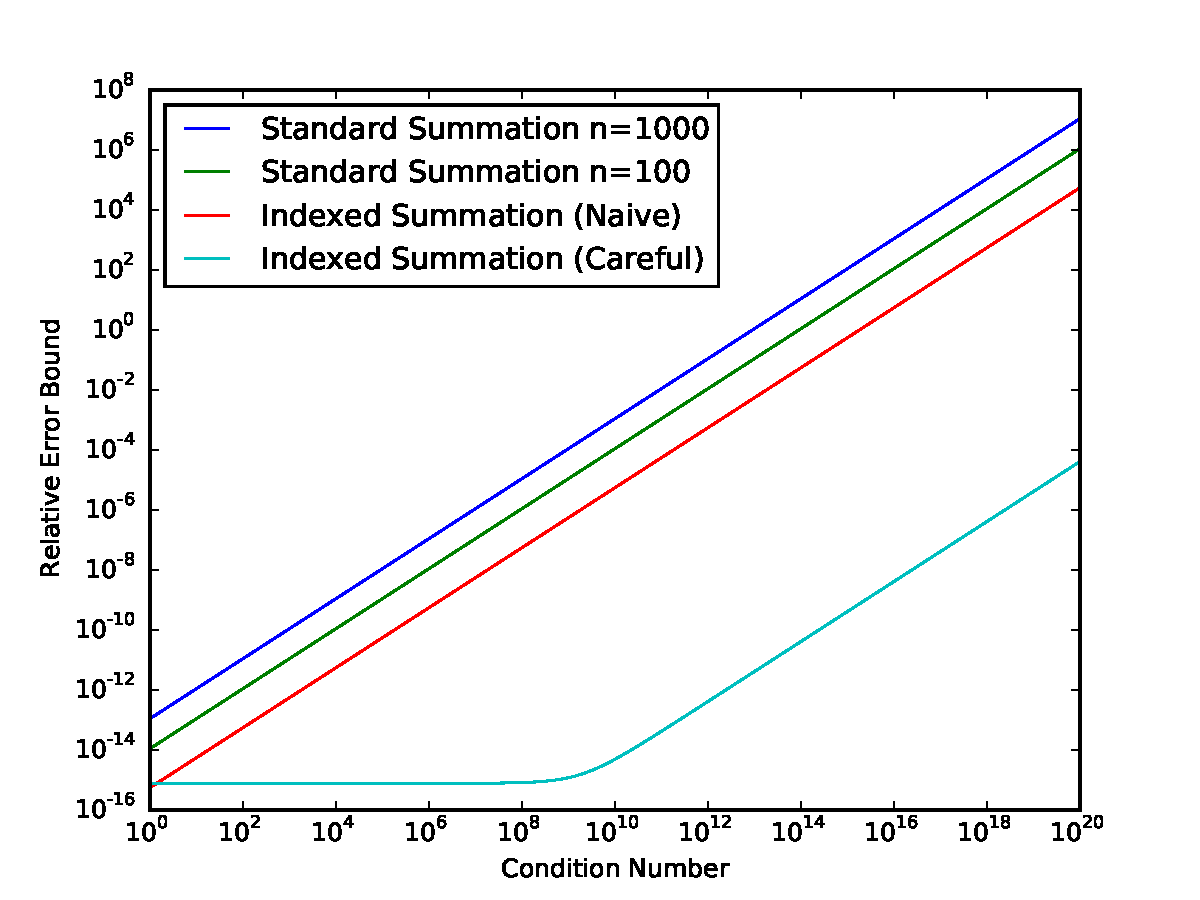
\includegraphics[width=\textwidth]{plots/errorcomparison.pdf}
\caption{Relative error bounds in calculating $|\sum \limits_{j = 0}^{n - 1}
x_j|$ for different condition numbers (which we define as $\frac{n \cdot \max
|x_j|)}{|\sum \limits_{j = 0}^{n - 1} x_j|}$) of the sum. It is assumed that we
sum using \texttt{double}, $K = 3$, and $W = 40$. ``Indexed Summation
(Careful)'' corresponds to \eqref{eq:errorapproxdup}. ``Indexed Summation
(Naive)'' corresponds to \eqref{eq:baderrorapproxdup}. ``Standard Summation''
corresponds to \eqref{eq:naiveerrorapproxdup} and due to a dependence on $n$
multiple error bounds are shown.}
\label{fig:conversionmotivation}
\end{center}
\end{figure}

    Next we show how to interpret the fields as unnormalized floating point numbers,
    and sort their exponents independently of the actual values of the fields.
    Note that, this interpretation is to support reasoning the conversion algorithm
    presented below, and is not used to change the representation format of the data itself
    since IEEE floating-point formats do not permit unnormalized numbers
    beside exeptional values and subnormals.
    Consider a $K$-fold indexed type $Y$ of index $I$.
    As each value ${\mathcal{Y}_k}_P$ in a primary field ${Y_k}_P$ is represented by an offset from $1.5  \epsilon^{-1}  2^{a_{I + k}}$ and ${Y_k}_P \in (\epsilon^{-1}  2^{a_{I + k}}, 2  \epsilon^{-1}  2^{a_{I + k}})$, ${\mathcal{Y}_k}_P$ can be expressed exactly using an unnormalized floating point number ${\mathcal{Y}'_P}_k$ with an exponent of $a_{I + k} + p - 1$.
    As each carry field ${Y_k}_C$ is a count of renormalization adjustments later scaled by $0.25  \epsilon^{-1}  2^{a_{I + k}}$, ${\mathcal{Y}_k}_C$ can be expressed exactly using an unnormalized floating point number ${\mathcal{Y}'_k}_C$ with an exponent of $a_{I + k} + 2  p - 3$.

    First, we have $\exp({\mathcal{Y}'_k}_P) > \exp({\mathcal{Y}'_{k+1}}_P)$ and $\exp({\mathcal{Y}'_{k}}_C) > \exp({\mathcal{Y}'_{k+1}}_C)$ because $a_{I + k} > a_{I + k+1}$.

    Next, note that
    \begin{equation*}
      \exp({\mathcal{Y}'_k}_C) = a_{I + k} + 2  p - 3
    \end{equation*}

    and
    \begin{equation*}
      \exp({\mathcal{Y}'_{k - 1}}_P) = a_{I + k - 1} + p - 1 = a_{I + k} + W + p - 1
    \end{equation*}

    Therefore $\exp({\mathcal{Y}'_k}_C) > \exp({\mathcal{Y}'_{k - 1}}_P)$ because $W < p - 2$.

    Finally, note that
    \begin{equation*}
      \exp({\mathcal{Y}'_{k - 2}}_P) = a_{I + k - 1} + p - 1 = a_{I + k} + 2 W + p - 1
    \end{equation*}

    Therefore $\exp({\mathcal{Y}'_k}_C) < \exp({\mathcal{Y}'_{k - 2}}_P)$ because $2  W > p + 1$.

    Combining the above inequalities, we see that the exponents of all the ${\mathcal{Y}'_k}_P$ and ${\mathcal{Y}'_k}_C$ are distinct and can be sorted as follows:

    \begin{alignat*}{5}
    \exp({\mathcal{Y}'_0}_C) &> \exp({\mathcal{Y}'_1}_C) &&> \exp({\mathcal{Y}'_0}_P) &&> \exp({\mathcal{Y}'_2}_C) &&> \exp({\mathcal{Y}'_1}_P) &&> ... \\
    ... &> \exp({\mathcal{Y}'_k}_C) &&> \exp({\mathcal{Y}'_{k - 1}}_P) &&> \exp({\mathcal{Y}'_{k + 1}}_C) &&> \exp({\mathcal{Y}'_k}_P) &&> ... \\
    ... &> \exp({\mathcal{Y}'_{K - 2}}_C) &&> \exp({\mathcal{Y}'_{K - 3}}_P) &&> \exp({\mathcal{Y}'_{K - 1}}_C) &&> \exp({\mathcal{Y}'_{K - 2}}_P) &&> \exp({\mathcal{Y}'_{K - 1}}_P)
    \end{alignat*}


    These unnormalized floating point numbers may, for convenience of notation,
    be referred to in decreasing order of unnormalized exponent as $\gamma'_0,
    ..., \gamma'_{2  K - 1}$.

    We have just shown that
    \begin{equation}
      \exp(\gamma_0') > ... > \exp(\gamma_{2  K - 1}')
      \label{eq:gammadecreases}
    \end{equation}
    where $\gamma_j$ denotes the normalized representation of the $\gamma'_j$.
    It should be noted that $\gamma_j = \gamma'_j$ as real numbers and that
    $\exp(\gamma_j) \leq \exp(\gamma'_j)$.

    It should be noted that if $\gamma_j$ is a primary field, then either
    $\gamma_{j + 1}$ or $\gamma_{j + 2}$ is a primary field (with the exception of $\gamma_{2K-1}$).
    If $\gamma_j$ is a
    carry field, then either $\gamma_{j + 1}$ or $\gamma_{j + 2}$ is a carry
    field (with the exception of $\gamma_{2  K - 3}$,
    but in this case, suppose that $p \geq 5$ which is true for both IEEE double and single precision,
    we have
    \(
        \exp(\gamma_{2  K - 3}')
        = a_{I + K - 1} + 2  p - 3 \geq a_{I + K - 1} + p + \lceil\frac{p + 1}{2}\rceil - 1
        = \exp(\gamma_{2  K - 1}') + \lceil\frac{p + 1}{2}\rceil
    \)
    ).
    Therefore, as $2  W > p + 1$, for all $j \in \{0, ..., 2K - 3\}$
    \begin{equation}
      \exp(\gamma_j') \geq \exp(\gamma_{j + 2}') + W \geq \exp(\gamma_{j + 2}') + \left\lceil\frac{p + 1}{2}\right\rceil
      \label{eq:gammadecreasesfast}
    \end{equation}

    It should be noted that the ${\mathcal{Y}'_k}_P$ and the
    ${\mathcal{Y}'_k}_C$ can be expressed exactly using floating point types of
    the same precision as ${Y_k}_P$ and ${Y_k}_C$ (except in the case of
    overflow, in which a scaled version may be obtained), and such exact
    floating point representations can be obtained using  \eqref{eq:pri} and
    \eqref{eq:car}.

    Now that we know how to obtain sorted, possibly scaled, fields in order of
    decreasing unnormalized exponent, we explain how to sum them while avoiding
    overflow. We will refer to the floating point type that we use to hold the
    sum during computation as the \textbf{intermediate} floating point type.
    Such a type must have at least as much precision and exponent range as the
    original floating point type.

    Notice that $|\gamma'_0| = |{\mathcal{Y}'_0}_C| < 2 \cdot 2^{\exp({\mathcal{Y}'_0}_C)} = 2 \cdot 2^{e_{\max} + 1 - W + 2  p - 3}$ and $\exp(\gamma'_0) > ... > \exp(\gamma'_{2  K - 1})$.  Therefore $|\gamma'_j| \leq 2^{e_{\max} - W + 2  p - 1 - j}$. The absolute value represented by an indexed type can therefore be bounded by

    \begin{equation}
      \label{eq:maxindexedvalue}
      \sum\limits_{j = 0}^{2  K - 1} |\gamma_j| < \sum\limits_{j = 0}^{2  K - 1} 2^{e_{\max} - W + 2  p - 1 - j} < \sum\limits_{j = 0}^{\infty} 2^{e_{\max} - W + 2  p - 1 - j} = 2^{e_{\max} - W + 2  p}
    \end{equation}

    If the intermediate floating point type has a maximum exponent greater than
    or equal to $e_{\max} - W + 2  p - 1$, then no special cases to guard
    against overflow are needed.

    Algorithm \ref{alg:conv2float} represents a conversion routine in such a case.

    \begin{samepage}
    \begin{alg}
      Convert $K$-fold indexed type $Y$ of index $I$ to floating point $x$.
      Here, $z$ is a floating point type with at least the original precision
      and maximum exponent $E_{\max}$ greater than $e_{\max} - W + 2  p$
      \begin{algorithmic}[1]
        \Function{ConvertIndexedToFloat}{K, x, Y}
          \If {${\mathcal{Y}_0}_C$ is NaN or $\pm$Inf}
            \State $x = {\mathcal{Y}_0}_C$
            \State \Return
          \EndIf
          \State $z = {\mathcal{Y}_0}_C$
          \For{$k = 1 \To K - 1$}
            \State $z = z + {\mathcal{Y}_k}_C$
            \State $z = z + {\mathcal{Y}_{k - 1}}_P$
          \EndFor
          \State $z = z + {\mathcal{Y}_{K - 1}}_P$
          \State $x = z$ \label{alg:conv2float:conv}
        \EndFunction
      \end{algorithmic}
      \label{alg:conv2float}
    \end{alg}
    \end{samepage}

    Note that an overflow situation in Algorithm \ref{alg:conv2float} is
    reproducible as the fields in $Y$ are reproducible. $z$ is
    deterministically computed from the fields of $Y$, and the condition that
    $z$ overflows when being converted back to the original floating point type
    in line \ref{alg:conv2float:conv} is reproducible.

    If an intermediate floating point type with exponent greater than or equal
    to $e_{\max} - W + 2  p - 1$ is not available and the lowest bin has index
    0, a rare case, the $\gamma_j$ must be scaled down by some factor during
    addition and the sum scaled back up when subsequent additions can no longer
    effect an overflow situation.

    If the scaled sum is to overflow, then its unscaled value will be greater
    than or equal to $2 \cdot 2^{e_{\max}}$ and it will overflow regardless of
    the values of any ${\mathcal{Y}_k}_P$ or ${\mathcal{Y}_k}_C$ with
    $|{\mathcal{Y}_k}_P| < 0.5 \cdot 2^{-\rho} 2^{e_{\max}}$ or
    $|{\mathcal{Y}_k}_C| < 0.5 \cdot 2^{-\rho}2^{e_{\max}}$ (where $\rho$ is
    the intermediate floating point type's precision). If the floating point
    sum has exponent greater than or equal to $e_{\max}$ these numbers are not
    large enough to have any effect when added to the sum. If the sum has
    exponent less than $e_{\max}$, then additions of these numbers cannot cause
    the exponent of the sum to exceed $e_{\max}$ for similar reasons.

    As the maximum absolute value of the true sum is strictly smaller than
    $2^{e_{\max} - W + 2 p}$, a sufficient scaling factor is $2^{2p-W-2}$,
    meaning that the maximum absolute value of the true scaled sum is
    strictly smaller $2 \cdot 2^{e_{\max} - 1}$ (and since it will be shown
    later that the computed sum is accurate to within a small factor of the
    true sum, the computed sum will stay strictly smaller than $2 \cdot
    2^{e_{\max}}$ and will not overflow.)

    When $\exp(\gamma'_j) < e_{\max} - \rho - 1$, the sum may be scaled back up
    and the remaining numbers added without scaling. Notice that no overflow
    can occur during addition in this algorithm. If an overflow is to occur, it
    will happen only when scaling back up. As the fields in the indexed type
    are reproducible, such an overflow condition is reproducible.

    If the sum is not going to overflow, then the smaller $y'_j$ must be added
    as unscaled numbers to avoid underflow.

    Algorithm \ref{alg:conv2floatoverflow} represents a conversion routine in such a case.

    \begin{samepage}
    \begin{alg}
      Convert a $K$-fold indexed type $Y$ of index $I$ to floating point $x$.
      Here, $z$ is a floating point number with precision $\rho \geq p$
      \begin{algorithmic}[1]
        \Function{ConvertIndexedToFloat0}{K, x, Y}
          \If {${\mathcal{Y}_0}_C$ is NaN or $\pm$Inf}
            \State $x = {\mathcal{Y}_0}_C$
            \State \Return
          \EndIf
          \State $k = 1$
          \While{$k \leq 2 K$ and $\exp(\gamma_k) \geq e_{\max} - \rho - 1$}
            \State $z = z + (\gamma_k / 2^{2 p - W - 2})$
            \State $k = k + 1$
          \EndWhile
          \State $z = z \cdot 2^{2 p - W - 2}$
          \While{$k \leq 2 K$}
            \State $z = z + \gamma_k$
            \State $k = k + 1$
          \EndWhile
          \State $x = z$
        \EndFunction
      \end{algorithmic}
      \label{alg:conv2floatoverflow}
    \end{alg}
    \end{samepage}

    If an indexed type is composed of \texttt{float}, then \texttt{double}
    provides sufficient precision and exponent to use as an intermediate type
    and Algorithm \ref{alg:conv2float} may be used to convert to a floating
    point number.  However, if an indexed type is composed of \texttt{double},
    many machines may not have any higher precision available. We therefore
    perform the sum using \texttt{double} as an intermediate type. As this does
    not extend the exponent range we must use Algorithm
    \ref{alg:conv2floatoverflow} for the conversion.

  \subsection{Error Bound}
    \label{sec:primitiveops_error}

    We first state and prove Theorem \ref{thm:mysortsum}, as it is critical in
    the error analysis of the algorithm. It should be noted that Theorem
    \ref{thm:mysortsum} is similar to that of Theorem 1 from \cite{sortsum},
    but requires less intermediate precision by exploiting additional structure
    of the input data.

    It is possible that future implementors may make modifications to the
    indexed type (adding multiple carry fields, changing the binning scheme,
    etc.) such that the summation of its fields cannot be reordered to satisfy
    the assumptions of Theorem \ref{thm:mysortsum}. In such an event,
    $\cite{sortsum}$ provides more general ways to sum the fields while still
    maintaining accuracy.
      \begin{samepage}
    \begin{thm}
      We are given $n$ floating point numbers $f_0, \ldots, f_{n - 1}$ for which there
      exist (possibly unnormalized) floating point numbers $f'_0, \ldots, f'_{n -1}$
      of the same precision such that
      \begin{enumerate}
        \item $f_j = f'_j$ for all $j \in \{0, ..., n - 1\}$
        \item $\exp(f'_0) > ... > \exp(f'_{n - 1})$
        \item $\exp(f'_j) \geq \exp(f'_{j + 2}) + \lceil\frac{p + 1}{2}\rceil$ for all $j \in \{0, ..., n - 3\}$
      \end{enumerate}
      \label{thm:mysortsum}
      Let $S_0 = \overline{S_0} = f_0$, $S_j = S_{j - 1} + f_j$,
      and $\overline{S_j} = \fl(\overline{S_{j - 1}} + f_j)$ (assuming rounding to nearest)
      so that $S_{n - 1} = \sum \limits_{j = 0}^{n - 1} f_j$.
      Then in the absence of overflow and underflow we have
      \begin{equation*}
        \left|S_{n - 1} - \overline{S_{n - 1}}\right| < \frac{7\epsilon}{1 - 6\sqrt\epsilon}|S_{n - 1}| \approx 7 \epsilon |S_{n - 1}|
      \end{equation*}
    \end{thm}
    \end{samepage}

    \begin{proof}

      Throughout the proof, let $f_j = 0$ if $j > n - 1$ so that $S_{\infty} = S_{n - 1}$ and $\overline{S_{\infty}} = \overline{S_{n - 1}}$.

      Let $m$ be the location of the first error such that $S_{m - 1} = \overline{S_{m - 1}}$ and $S_{m} \neq \overline{S_{m}}$.

      If no such $m$ exists then the computed sum is exact ($S_{n - 1} = \overline{S_{n - 1}}$) and we are done.

      If such an $m$ exists, then because $\exp(f_0') > ... > \exp(f_m')$, $f_0, ..., f_m \in \ulp(f_m')\Z$. Thus, $S_m \in \ulp(f_m')\Z$.

      We now show $|S_m| > 2 \cdot 2^{\exp(f_m')}$. Assume for contradiction that $|S_m| \leq 2 \cdot 2^{\exp(f_m')}$. Because $S_m \in \ulp(f_m')\Z$, this would imply that $S_m$ is representable as a floating point number, a contradiction as $\overline{S_m} \neq S_m$. Therefore, we have
      \begin{equation}
        |S_m| > 2 \cdot 2^{\exp(f_m')}
        \label{eq:smbound}
      \end{equation}

      Because $\exp(f_m') > \exp(f_{m + 1}')$,
      \begin{equation}
        |f_{m + 1}| < 2\cdot2^{\exp(f_m' - 1)} = 2^{\exp(f_m')}
        \label{eq:smpbound}
      \end{equation}

      Because $\exp(f_m') \geq \exp(f_{m + 2}') + \lceil\frac{p + 1}{2}\rceil$ and $\exp(f_0') > ... > \exp(f_{n - 1}')$,
      \begin{align}
        \bigl|\sum \limits_{j = m + 2}^{n - 1} f_j\bigr| &\leq \sum \limits_{j = m + 2}^{n - 1} |f_j| < \sum \limits_{j = m + 2}^{n - 1} 2 \cdot 2^{\exp(f_j')} \leq \sum \limits_{j = m + 2}^{n - 1} 2 \cdot 2^{\exp(f_m') - \left\lceil\frac{p + 1}{2}\right\rceil - (m + 2 - j)} \nonumber \\
        &< \sum \limits_{j = 0}^{\infty} \left(2 \sqrt{\epsilon}\right)2^{\exp(f_m') - j} = \left(4\sqrt\epsilon\right)2^{\exp(f_m')}
        \label{eq:smppbound}
      \end{align}

      We can combine  \eqref{eq:smpbound} and \eqref{eq:smppbound} to obtain
      \begin{equation}
        \bigl|\sum\limits_{j = m + 1}^{n - 1} f_j\bigr| \leq \sum\limits_{j = m + 1}^{n - 1} |f_j| < 2^{\exp{f_m'}} + \left(4 \sqrt{\epsilon}\right) 2^{\exp(f_m')} = \left(1 + 4 \sqrt\epsilon \right)2^{\exp(f_m')}
        \label{eq:smsbound}
      \end{equation}

      By  \eqref{eq:smbound} and \eqref{eq:smsbound},
      \begin{align}
        |S_{n-1}| & = \bigl|\sum\limits_{j = 0}^{n - 1} f_j\bigr| \geq \bigl|\sum\limits_{j = 0}^{m} f_j\bigr| - \bigl|\sum\limits_{j = m + 1}^{n - 1} f_j\bigr| = |S_m| - \bigl|\sum\limits_{j = m + 1}^{n - 1} f_j\bigr| \nonumber \\
        & \geq 2 \cdot 2^{\exp(f_{m}')} - \left(1 + 4 \sqrt\epsilon\right) 2^{\exp(f_m')} = \left(1 - 4 \sqrt\epsilon\right) 2^{\exp(f_m')}
        \label{eq:sbound}
      \end{align}

      By  \eqref{eq:sbound} and \eqref{eq:smppbound},
      \begin{equation}
        \bigl|\sum \limits_{j = m + 2}^{n - 1} f_j\bigr| < \left(4 \sqrt{\epsilon}\right) 2^{\exp(f_m')} \leq \frac{4 \sqrt\epsilon}{1 - 4  \sqrt\epsilon}\bigl|\sum\limits_{j = 0}^{n - 1}f_j\bigr|
        \label{eq:smpprelsbound}
      \end{equation}

      By  \eqref{eq:sbound} and \eqref{eq:smsbound},
      \begin{equation}
        \bigl|\sum\limits_{j = m + 1}^{n - 1}f_j\bigr| \leq \sum\limits_{j = m + 1}^{n - 1}|f_j| \leq \left(1 + 4  \sqrt\epsilon\right)2^{\exp(f_m')}\leq \frac{1 + 4  \sqrt\epsilon}{1 - 4  \sqrt\epsilon}\bigl|\sum\limits_{j = 0}^{n - 1}f_j\bigr|
        \label{eq:smsrelsbound}
      \end{equation}

      And by \eqref{eq:sbound} and \eqref{eq:smsrelsbound},
      \begin{equation}
        |S_m| \leq \bigl|\sum\limits_{j = 0}^{n - 1}f_j\bigr| + \bigl|\sum\limits_{j = m + 1}^{n - 1} f_j\bigr|
            \leq \left(1 + \frac{1 + 4\sqrt\epsilon}{1 - 4\sqrt\epsilon}\right)\bigl|\sum_{j = 0}^{n - 1}f_j\bigr|
            = \frac{2}{1 - 4  \sqrt\epsilon}\bigl|\sum\limits_{j = 0}^{n - 1}f_j\bigr|
        \label{eq:smrelsbound}
      \end{equation}

      By definition, $\overline{S_{m+4}}$ is the computed sum of
      $\overline{S_m}$, $f_{m+1}, \ldots, f_{m+4}$ using the standard recursive summation technique.
      According to \cite[Equation 1.2, 2.4]{higham}
      \begin{align*}
          \bigl|\overline{S_m} + \sum_{j=m+1}^{m+4}f_j - \overline{S_{m+4}}\bigr|
          & \leq \frac{4\epsilon}{1-4\epsilon} \left|\overline{S_m} + f_{m+1}\right| + \frac{3\epsilon}{1-3\epsilon} \sum_{j=m+2}^{m+4}|f_j| \\
          & \leq \frac{4\epsilon}{1-4\epsilon} \bigl(\left|\overline{S_m} - S_m\right| + |S_m + f_{m+1}|\bigr)
              + \frac{3\epsilon}{1-3\epsilon} \sum_{j=m+2}^{n-1}|f_j|.
      \end{align*}
      Since $S_{n-1} = S_m + f_{m+1} + \sum_{j=m+2}^{n-1} f_j$, we have
      \begin{equation*}
          |S_m + f_{m+1}|
          = \bigl|S_{n-1} - \sum_{j=m+2}^{n-1}f_j\bigr|
          \leq |S_{n-1}| + \sum_{j=m+2}^{n-1} |f_j|
      \end{equation*}
      Therefore
      \begin{equation*}
          \bigl|\overline{S_m} + \sum_{j=m+1}^{m+4}f_j - \overline{S_{m+4}}\bigr|
          \leq \frac{4\epsilon}{1-4\epsilon} \left|S_m - \overline{S_m}\right|
          + \frac{4\epsilon}{1-4\epsilon} |S_{n-1}|
          + \frac{7\epsilon}{1-4\epsilon} \sum_{j=m+2}^{n-1}|f_j|.
      \end{equation*}
      Using the triangle inequality we have
      \begin{align*}
      \left|S_{m+4} - \overline{S_{m+4}}\right|
          & = \bigl|S_m + \sum_{j=m+1}^{m+4}f_j - \overline{S_{m+4}}\bigr|
          \leq \left|S_m - \overline{S_m} \right| + \bigl|\overline{S_m} + \sum_{j=m+1}^{m+4}f_j - \overline{S_{m+4}} \bigr| \\
          & \leq \left(1 + \frac{4\epsilon}{1-4\epsilon}\right) \left|S_m - \overline{S_m}\right| + \frac{4\epsilon}{1-4\epsilon} |S_{n-1}|
                  + \frac{7\epsilon}{1-4\epsilon} \sum_{j=m+2}^{n-1}|f_j| \\
          & \leq \frac{1}{1-4\epsilon} \epsilon |S_m| + \frac{4\epsilon}{1-4\epsilon} |S_{n-1}|
                  + \frac{7\epsilon}{1-4\epsilon} \sum_{j=m+2}^{n-1}|f_j| \\
          & \leq \frac{\epsilon}{1-4\epsilon} \left(|S_m| + 4 |S_{n-1}|
                  + 7 \sum_{j=m+2}^{n-1}|f_j|\right).
      \end{align*}
      and by \eqref{eq:smrelsbound} and \eqref{eq:smpprelsbound},
      \begin{align}
      \left|S_{m+4} - \overline{S_{m+4}}\right|
          & \leq \frac{\epsilon}{1-4\epsilon}
              \left(
                  \frac{2}{1-4\sqrt{\epsilon}} |S_{n-1}|
                  + 4 |S_{n-1}|
                  + 7 \frac{4\sqrt{\epsilon}}{1-4\sqrt{\epsilon}} |S_{n-1}|
              \right) \nonumber \\
          & \leq \frac{\epsilon}{1-4\epsilon} \left(\frac{6+12\sqrt{\epsilon}}{1-4\sqrt{\epsilon}} |S_{n-1}|\right)
              = \frac{6\epsilon }{(1-2\sqrt{\epsilon})(1-4\sqrt{\epsilon})} |S_{n-1}| \nonumber \\
          & < \frac{6\epsilon}{1-6\sqrt{\epsilon}} |S_{n-1}|
          \label{eq:smfiveerror}
      \end{align}

      Notice that
      \begin{equation*}
        \exp(f_m') \geq \exp(f_{m + 2}') + \left\lceil\frac{p+ 1}{2}\right\rceil \geq \exp(f_{m + 4}') + 2  \left\lceil\frac{p + 1}{2}\right\rceil > \exp(f_{m + 5}')+ 2  \left\lceil\frac{p+ 1}{2}\right\rceil
      \end{equation*}
      Therefore,
      \begin{equation}
        \exp(f_m') \geq \exp(f_{m + 5}') + p + 2
        \label{eq:fmfiveexp}
      \end{equation}

      Because $\exp(f_0') > ... > \exp(f_{n - 1}')$, \eqref{eq:fmfiveexp} yields
      \begin{equation}
        \bigl|\sum\limits_{j = m + 5}^{n - 1} f_j\bigr| \leq \sum\limits_{j = m + 5}^{n - 1} |f_j| < \sum\limits_{j = m + 5}^{n - 1} 2 \cdot 2^{\exp(f_m') - p - 2 - (j - (m + 5))} < \sum\limits_{j = 0}^{\infty} 2^{\exp(f_m') - p - 1 - j} = \epsilon 2^{\exp(f_m')}
        \label{eq:boundfmfivesum}
      \end{equation}

      Using \eqref{eq:sbound} and \eqref{eq:boundfmfivesum},
      \begin{equation}
        \bigl|\sum\limits_{j = m + 5}^{n - 1} f_j\bigr| \leq \sum\limits_{j = m + 5}^{n - 1} |f_j| < \frac{\epsilon}{1 - 4  \sqrt\epsilon}|S_{n - 1}|
        \label{eq:relsboundfmfivesum}
      \end{equation}

      By \eqref{eq:smfiveerror} and \eqref{eq:relsboundfmfivesum}
      \begin{align}
        \left|S_{n-1} - \overline{S_{m+4}}\right|
        & \leq |S_{n-1} - S_{m+4}| + \left|S_{m+4} - \overline{S_{m+4}}\right| \nonumber \\
        & \leq \bigl|\sum_{j=m+5}^{n-1} f_j\bigr| + \frac{6\epsilon}{1-6\sqrt{\epsilon}} |S_{n-1}| \nonumber \\
        & \leq \frac{\epsilon}{1 - 4 \sqrt\epsilon}|S_{n-1}| + \frac{6\epsilon}{1-6\sqrt{\epsilon}} |S_{n-1}| \nonumber \\
        & <  \frac{7\epsilon}{1-6\sqrt{\epsilon}} |S_{n-1}|.
        \label{eq:smfiveerror-1}
      \end{align}

      When combined with \eqref{eq:sbound} this gives
      \begin{align*}
        \left|\overline{S_{m+4}}\right|
        & \geq \left(1-\frac{7 \epsilon}{1-6\sqrt{\epsilon}}\right) |S_{n-1}| \\
        & > \left(1-\frac{7 \epsilon}{1-6\sqrt{\epsilon}}\right) \left(1-4\sqrt{\epsilon}\right) 2^{\exp(f'_m)} \\
        & > \left(1-4\sqrt{\epsilon} - \frac{7 \epsilon \left(1-4\sqrt{\epsilon}\right)}{1-6\sqrt{\epsilon}}\right) 2^{\exp(f'_m)}
      \end{align*}

      which, assuming $\epsilon \ll 1$, can be simplified to
      \begin{equation}
        \left|\overline{S_{m + 4}}\right| > 2^{\exp(f_m') - 1}
        \label{eq:minsmfoursimple}
      \end{equation}

      Using  \eqref{eq:fmfiveexp}, for all $j \geq m + 5$ we have
      \begin{equation}
        |f_j| < 2 \cdot 2^{\exp(f_j')} \leq 2 \cdot 2^{\exp(f_m') - p - 2} = \epsilon \cdot 2^{\exp(f_m') - 1}
        \label{eq:maxfmfive}
      \end{equation}

      And by \eqref{eq:maxfmfive} and \eqref{eq:minsmfoursimple}, all additions
      after $f_{m + 4}$ have no effect (since we are rounding to nearest)
      and we have $\overline{S_{n-1}} = \overline{S_{m+4}}$.
      This, together with \eqref{eq:smfiveerror-1}, implies
      \begin{equation*}
        \left|S_{n-1} - \overline{S_{n-1}}\right| < \frac{7\epsilon}{1-6\sqrt{\epsilon}} |S_{n-1}|
      \end{equation*}
      The proof is complete.
    \end{proof}

    Consider the $K$-fold indexed sum $Y$ of floating point numbers $x_0, \ldots, x_{n - 1}$.
    We denote the true sum $\sum \limits_{j = 0}^{n - 1} x_j$ by $T$, the true
    value of the indexed sum as obtained using \eqref{eq:indexedvalue} by
    $\mathcal{Y}$, and the floating point approximation of $\mathcal{Y}$
    obtained using an appropriate algorithm from Section
    \ref{sec:primitiveops_convert} by $\overline{\mathcal{Y}}$.

    \cite{repsum} discusses the absolute error $|T - \mathcal{Y}|$ but does not
    give a method to construct $\overline{\mathcal{Y}}$ and therefore no error
    bound $|T - \overline{\mathcal{Y}}|$ on the final floating point answer
    was given. Here we extend the error bound of \cite{repsum} all the way to
    the final return value of the algorithm.

    %It has been shown in \cite{repsum} that
    The case of all zero input data is trivial, therefore we assume that
    $\max|x_j|$ and $Y$ are nonzero.
    We also assume here no overflow or underflow.
    Let $I$ be the index of $Y$, which is also the index of $\max|x_j|$,
    so that $2^{b_I} > \max|x_j| \geq 2^{a_I}$.
    Therefore for all $i < I$ the slice of any $x_j$ in bin $i$ is $d(x_j, i) = 0$.
    The index of the smallest bin of $Y$ is $I + K - 1$.
    According to Theorem~\ref{thm:dround}, we have
    \begin{align*}
        |x_j - \sum_{i=I}^{I + K -1} d(x_j,i)|
            & = |x_j - \sum_{i=0}^{I + K - 1} d(x_j,i)|
            \leq 2^{a_{I + K -1}} 
            = 2^{a_I - (K-1)W} \\
            & \leq 2^{W(1-K)} \max|x_j|. 
    \end{align*}

    Since the summation in each bin $Y_i$ is exact, we have
    \begin{align}
        |T - \mathcal{Y}| & = |\sum_{j=0}^{n-1} x_j - \sum_{i=I}^{I+K-1} \sum_{j=0}^{n-1} d(x_j, i)|
            = |\sum_{j=0}^{n-1} (x_j - \sum_{i=I}^{I+K-1} d(x_j,i))| \nonumber \\
            & \leq n 2^{W(1-K)} \max|x_j|.
            \label{eq:repboundnaive}
    \end{align}

    However, this bound does not consider underflow. By
    \eqref{eq:droundunderflow}, a small modification yields a bound that
    considers underflow
    \begin{equation}
      \label{eq:repbound}
      |T - \mathcal{Y}| < n \cdot \max\bigl(2^{W  (1 - K)} \max|x_j|, 2^{e_{\min} - 1}\bigr)
    \end{equation}

    By  \eqref{eq:gammadecreases} and \eqref{eq:gammadecreasesfast},
    Theorem \ref{thm:mysortsum} applies to yield
    \begin{equation*}
      \left|\mathcal{Y} - \overline{\mathcal{Y}}\right| < \frac{7\epsilon}{1 - 6\sqrt\epsilon}|\mathcal{Y}|
    \end{equation*}

    By the triangle inequality
    \begin{equation*}
      |\mathcal{Y}| \leq |T| + |T - \mathcal{Y}| < n \cdot \max\bigl(2^{W(1-K)}  \max|x_j|, 2^{e_{\min} - 1}\bigr) + |T|
    \end{equation*}

    The above results can be used to obtain  \eqref{eq:error}, the absolute
    error of the floating point approximation of an indexed sum $|T - \overline{\mathcal{Y}}|$.
    \begin{align}
      \left|T - \overline{\mathcal{Y}}\right| &\leq |T - \mathcal{Y}| + \left|\mathcal{Y} - \overline{\mathcal{Y}}\right| \nonumber \\
      &< n \cdot \max\bigl(2^{W  (1 - K)}  \max|x_j|, 2^{e_{\min} - 1}\bigr) + \frac{7\epsilon}{1 - 6\sqrt\epsilon} |\mathcal{Y}| \nonumber \\
      &< n \cdot \max\bigl(2^{W  (1 - K)}  \max|x_j|, 2^{e_{\min} - 1}\bigr) \nonumber \\
      &+ \frac{7\epsilon}{1 - 6\sqrt\epsilon} \Bigl(n \cdot \max\bigl(2^{W  (1 - K) - 1}  \max|x_j|, 2^{e_{\min} - 1}\bigr) + |T|\Bigr) \nonumber \\
      &< \left(1 + \frac{7\epsilon}{1 - 6\sqrt\epsilon}\right) \Bigl(n \cdot \max\bigl(2^{W (1 - K)} \max|x_j|, 2^{e_{\min} - 1}\bigr)\Bigr) + \frac{7\epsilon}{1 - 6\sqrt\epsilon} |T|
      \label{eq:error}
    \end{align}

    Equation \eqref{eq:error} can be approximated as \eqref{eq:errorapprox}:
    \begin{align}
      \left|T - \overline{\mathcal{Y}}\right| &< \left(1 + \frac{7\epsilon}{1 - 6\sqrt\epsilon}\right) \Bigl(n \cdot \max\bigl(2^{W (1 - K)} \max|x_j|, 2^{e_{\min} - 1}\bigr)\Bigr) + \frac{7\epsilon}{1 - 6\sqrt\epsilon} |T| \nonumber \\
    &\approx n 2^{W  (1 - K)} \max|x_j| + 7  \epsilon |T|
      \label{eq:errorapprox}
    \end{align}

    A perhaps more useful mathematical construction is the error expressed
    relative to the result $\overline{\mathcal{Y}}$, and not the theoretical
    sum $T$. Again by the triangle inequality,
    \begin{equation*}
      |\mathcal{Y}| \leq \left|\overline{\mathcal{Y}}\right| + \left|\mathcal{Y} - \overline{\mathcal{Y}}\right|
    \end{equation*}

    Applying the bound on $|\mathcal{Y} - \overline{\mathcal{Y}}|$ yields
    \begin{equation*}
      |\mathcal{Y}| < \left|\overline{\mathcal{Y}}\right| + \frac{7\epsilon}{1 - 6\sqrt\epsilon}|\mathcal{Y}|
    \end{equation*}

    After simplification,
    \[
      |\mathcal{Y}| < \left(\frac{1}{1 - \frac{7\epsilon}{1 - 6\sqrt\epsilon}}\right)  \left|\overline{\mathcal{Y}}\right| \nonumber 
      = \frac{1 - 6 \sqrt\epsilon}{1 - 6 \sqrt \epsilon - 7\epsilon}  \left|\overline{\mathcal{Y}}\right|.
    \]

    The above results can be used to obtain  \eqref{eq:error2}, the absolute
    error of the floating point approximation of an indexed sum $|T -
    \overline{\mathcal{Y}}|$.
    \begin{align}
      \left|T - \overline{\mathcal{Y}}\right| &\leq |T - \mathcal{Y}| + \left|\mathcal{Y} - \overline{\mathcal{Y}}\right| \nonumber \\
      &< n \cdot \max\bigl(2^{W(1-K)}  \max|x_j|, 2^{e_{\min} - 1}\bigr) + \frac{7\epsilon}{1 - 6\sqrt\epsilon}|\mathcal{Y}| \nonumber \\
      &< n \cdot \max\bigl(2^{W(1-K)}  \max|x_j|, 2^{e_{\min} - 1}\bigr) + \frac{7\epsilon}{1 - 6\sqrt\epsilon}\left(\frac{1 - 6 \sqrt\epsilon}{1 - 6 \sqrt \epsilon - 7\epsilon}\left|\overline{\mathcal{Y}}\right|\right) \nonumber \\
      &= n \cdot \max\bigl(2^{W(1-K)}  \max|x_j|, 2^{e_{\min} - 1}\bigr) + \frac{7\epsilon}{1 - 6 \sqrt \epsilon - 7\epsilon}\left|\overline{\mathcal{Y}}\right|
      \label{eq:error2}
    \end{align}

    Equation \eqref{eq:error2} can be approximated as \eqref{eq:error2approx},
    which is nearly equal to bound \eqref{eq:errorapprox}:
    \begin{align}
      |T - \overline{\mathcal{Y}}| &< n \cdot \max\bigl(2^{W(1-K)}  \max|x_j|, 2^{e_{\min} - 1}\bigr) + \frac{7\epsilon}{1 - 6 \sqrt \epsilon - 7\epsilon}  \left|\overline{\mathcal{Y}}\right| \nonumber \\
      &\approx n  2^{W(1 - K)} \max|x_j|+ 7 \epsilon \left|\overline{\mathcal{Y}}\right|
      \label{eq:error2approx}
    \end{align}

    We can compare  \eqref{eq:errorapprox} to the error bound obtained if the
    accumulator fields were summed without extra precision. In this case, only
    the standard summation bound from \cite{higham} would apply and the
    absolute error would be bounded by
    \begin{equation*}
    n \cdot \max\bigl(2^{W(1-K)}  \max|x_j|, 2^{e_{\min} - 1}\bigr) + \left(\frac{(2  K - 1)  \epsilon}{1 - (2  K - 1)  \epsilon}\right)  \sum\limits_0^{2  K - 1}|\gamma_j|
    \end{equation*}
    which is approximately bounded by
    \begin{equation}
    n \cdot \max|x_j| \bigl(2^{W(1-K)} + (2  K - 1)  \epsilon\bigr)
    \label{eq:baderrorapprox}
    \end{equation}

    This is not as tight a bound as \eqref{eq:errorapprox}, and grows linearly
    as the user increases $K$ in an attempt to increase accuracy.

  \subsection{Limits}
    \label{sec:primitiveops_limits}
    As discussed previously, for a $K$-fold indexed type the minimum $K$
    accepted by ReproBLAS is 2. The maximum useful $K$ is
    $\lfloor(e_{\max} - e_{\min} + p - 1)/W\rfloor$,
    as this covers all of the bins.

    As discussed in \cite{repsum}, $W < p - 2$. As discussed in section
    \ref{sec:indexed_overflow}, $2 W > p + 1$.

    ReproBLAS uses the values $W = 40$ for indexed \texttt{double} and $W = 13$
    for indexed \texttt{float}. $W$ is available as the \texttt{XIWIDTH} macro.

    As discussed in section \ref{sec:indexed_underflow_gradual}, the input is
    rounded at best to the nearest $2^{e_{\min} - 1}$

    As absolute value of individual quantities added to ${Y_k}_P$ are not in
    excess of $2^{b_{I + k}}$, a maximum of $0.25\epsilon^{-1}2^{-W}$ elements
    may be deposited into ${Y_k}_P$ between renormalizations, as discussed in
    section \ref{sec:primitiveops_renormalize}. For indexed \texttt{double}
    this number is $2^{11}$, whereas for indexed \texttt{float} this number is
    $2^9$. This number is supplied programmatically using the
    \texttt{XIENDURANCE} macro.

    By \eqref{eq:totalfreq}, an indexed sum is capable of representing the sum
    of at least $0.25\epsilon^{-1}2^{-W}  (\epsilon^{-1} - 1) \approx 2^{2  p - W - 2}$
    floating point numbers. For indexed \texttt{double} this number is
    almost $2^{64}$, whereas for indexed \texttt{float} this number is almost
    $2^{33}$. This number is supplied programmatically using the
    \texttt{XICAPACITY} macro.

    The indexed types provided by ReproBLAS will, when used correctly, avoid intermediate overflow.

